\documentclass[12pt,a4paper]{report}

%\includeonly{cover/cimlap, chapters/1_introduction}

\usepackage{styles/dolgozat}

% folyamat- és szerkezeti ábrák (előfeldolgozás / modell fejezetek)
\usepackage{tikz}
\usetikzlibrary{positioning,arrows.meta,shapes.geometric}

% programkód beillesztéséhez
\usepackage{listings}
% listing float neve
\renewcommand{\lstlistingname}{Programkód}
%\renewcommand{\lstlistlistingname}{Programkódok listája}
%saját listings style-ok, és a style-t használó parancsok definíciói
\usepackage{styles/cpp}
\usepackage{styles/python}
%\usepackage{styles/java}
%\usepackage{styles/rust}

%% egyéb csomagok betöltése itt, vagy a dolgozat.sty fájlban

\usepackage{hyperref}
% cleveref csomag és beállításai -- az egyetlen, amit a hyperref után kell betölteni!
\usepackage{styles/refs}

\begin{document}

\pagestyle{empty}
\pagenumbering{gobble}

\begin{titlepage}
\centering
% A Miskolci Egyetem címere
\vspace*{2cm}
\huge\textsc{\textbf{Szakdolgozat}}\\[1cm]
%\vspace*{1cm}

\includegraphics[width=4.8cm, height=4cm,keepaspectratio]{images/me_logo.png}\\
\textbf{\textsc{Miskolci Egyetem}}

\vspace*{2cm}

% A szakdolgozat címe, akár több sorban is
{\LARGE\textbf{SPAM/HAM üzenetek osztályozása mélytanulási módszerekkel}}

\vspace*{2cm}
% A hallgató neve, évfolyam, szak(ok), a konzulens(ek) neve
\large
\textbf{Készítette:}\\[0.8ex]
Ferencsik Róbert\\[0.8ex]
Programtervező informatikus

\vspace*{0.5cm}
\textbf{Témavezető:}\\[0.8ex]
Dr. Baksáné Dr. Varga Erika

\vfill

% Keltezés: Hely, év
\large
\textbf{\textsc{Miskolc, 2026}}

\end{titlepage}
%Feladatkiiras
\noindent
\textsc{\textbf{Miskolci Egyetem}}\\
Gépészmérnöki és Informatikai Kar\\
Alkalmazott Matematikai Tanszék\hspace*{4cm}\hfil \textbf{Szám:}

\vspace{0.5cm}
\begin{center}
\large\textsc{\textbf{Szakdolgozat Feladat}}
\end{center}
\vspace{0.5cm}

Ferencsik Róbert (BQLOTW) BSc programtervező informatikus jelölt részére.

\bigskip
\noindent\textbf{A szakdolgozat tárgyköre:} gépi tanulás, klasszifikáció

\bigskip
\noindent\textbf{A szakdolgozat címe:} SPAM/HAM üzenetek és forráskódok osztályozása neurális hálók és nagy nyelvi modellek (LLM) segítségével

\bigskip
\noindent\textbf{A feladat részletezése:}

\medskip

\noindent A SPAM/HAM klasszifikációs feladat lényege annak eldöntése, hogy egy adott üzenet \emph{spam} (kéretlen, nem kívánt tartalom), vagy \emph{ham} (nem spam, hasznos tartalom). A probléma jól vizsgálható gépi tanulási és mélytanulási módszerekkel; különösen az LSTM (Long Short-Term Memory) architektúrák alkalmasak szekvenciális adatok---így szövegek---feldolgozására.

\medskip

\noindent A szakdolgozatban a hallgató először a SPAM/HAM osztályozást valósítja meg, majd a megközelítést kiterjeszti forráskódokra: a programkódokat \emph{malware} vagy \emph{benign} kategóriába kell sorolni.

\medskip

\noindent A modern nagy nyelvi modellek (LLM) lehetőséget adnak mind a természetes nyelvi szövegek, mind a programkódok szemantikai feldolgozására. A dolgozat célja az LSTM- és LLM-alapú megközelítések \emph{összehasonlítása} és \emph{teljesítményük értékelése} (megfelelő validációs és tesztelési protokoll mellett).

\vfill

\noindent\textbf{Témavezető(k):} Dr.\ Baksáné Dr.\ Varga Erika, egyetemi docens

\noindent\textbf{Konzulens(ek):}

\bigskip
\noindent\textbf{A feladat kiadásának ideje:} 2025.\ szeptember 9.

%\noindent\textbf{A feladat beadásának határideje:}

\vspace{1.5cm}

\hfill\makebox[6cm]{\dotfill}

\hfill\makebox[6cm]{szakfelelős}

\clearpage

\vspace*{1cm}  
\begin{center}
\large\textsc{\textbf{Eredetiségi Nyilatkozat}}
\end{center}
\vspace*{2cm}  

Alulírott \textbf{Ferencsik Róbert}; Neptun-kód: \texttt{BQLOTW} a Miskolci Egyetem Gépészmérnöki és Informatikai Karának végzős Programtervező informatikus szakos hallgatója ezennel büntetőjogi és fegyelmi felelősségem tudatában nyilatkozom és aláírásommal igazolom, hogy \textit{SPAM/HAM üzenetek és forráskódok osztályozása neurális hálók és nagy nyelvi modellek (LLM) segítségével}
című szakdolgozatom saját, önálló munkám; az abban hivatkozott szakirodalom
felhasználása a forráskezelés szabályai szerint történt.

\medskip
Tudomásul veszem, hogy szakdolgozat esetén plágiumnak számít:
\begin{itemize}
\item szószerinti idézet közlése idézőjel és hivatkozás megjelölése nélkül;
\item tartalmi idézet hivatkozás megjelölése nélkül;
\item más publikált gondolatainak saját gondolatként való feltüntetése.
\end{itemize}

Alulírott kijelentem, hogy a plágium fogalmát megismertem, és tudomásul veszem, hogy
plágium esetén szakdolgozatom visszautasításra kerül.

\vspace*{3cm}

\noindent Miskolc, \makebox[2cm]{\dotfill}. év \makebox[2cm]{\dotfill}. hó \makebox[2cm]{\dotfill}. nap

\vspace*{3cm}

\hfill\makebox[6cm]{\dotfill}

\hfill\makebox[6cm]{Hallgató}



\clearpage

\newcommand{\ki}{témavezető(k)}
\newsavebox{\alairas}
\begin{lrbox}{\alairas}
\begin{tabular}{c@{\hspace{2cm}}c}
\makebox[4cm]{\dotfill} & \makebox[5cm]{\dotfill} \\
dátum & \ki \\
\end{tabular}
\end{lrbox}
\newcommand{\dotline}{\makebox[5cm]{\dotfill}}
\newcommand{\shortdotline}{\makebox[3.5cm]{\dotfill}}

\noindent 1.
\begin{tabular}[t]{cl}
\multirow{2}{*}{A szakdolgozat feladat módosítása}
&szükséges (módosítás külön lapon) \\
& nem szükséges\\[1ex]
\end{tabular}

\begin{center}
\usebox{\alairas}
\end{center}

\smallskip

\noindent 2. A feladat kidolgozását ellenőriztem:

\begin{center}
\begin{tabular}{c@{\hspace*{2cm}}c}
témavezető (dátum, aláírás): & konzulens (dátum, aláírás):\\
\dotline & \dotline \\
\dotline & \dotline \\
\dotline & \dotline 
\end{tabular}
\end{center}

\smallskip

\noindent 3. A szakdolgozat beadható:

\begin{center}
\usebox{\alairas}
\end{center}

\noindent 4.
\begin{tabular}[t]{@{}l@{\hspace*{1mm}}l@{\hspace*{1mm}}l}
A szakdolgozat & \shortdotline & szövegoldalt\\
              & \shortdotline & program protokollt (listát, felhasználói leírást)\\
              & \shortdotline & elektronikus adathordozót (részletezve)\\
              & \shortdotline \\
              & \shortdotline & egyéb mellékletet (részletezve)\\
              & \shortdotline 
\end{tabular}
\newline tartalmaz.

\begin{center}
\usebox{\alairas}
\end{center}

\noindent 5.
\begin{tabular}[t]{ll}
\multirow{2}{*}{A szakdolgozat bírálatra} & bocsátható\\
& nem bocsátható\\
\end{tabular}

\smallskip

\noindent A bíráló neve: \makebox[8cm]{\dotfill}

\renewcommand{\ki}{szakfelelős}
\begin{center}
\begin{tabular}{c@{\hspace{2cm}}c}
\makebox[4cm]{\dotfill} & \makebox[5cm]{\dotfill} \\
dátum & \ki \\
\end{tabular}
\end{center}

\noindent 6.
\begin{tabular}[t]{lll}
A szakdolgozat osztályzata \\
& a témavezető javaslata: & \makebox[2.5cm]{\dotfill} \\
& a bíráló javaslata: & \makebox[2.5cm]{\dotfill} \\
& a szakdolgozat végleges eredménye: & \makebox[2.5cm]{\dotfill}
\end{tabular}

\bigskip\bigskip

\noindent Miskolc, \makebox[4cm]{\dotfill} \hfill \makebox[8cm]{\dotfill} 

\hfill \makebox[8cm]{a Záróvizsga Bizottság Elnöke} 


\tableofcontents

\clearpage
\pagenumbering{arabic}
\pagestyle{fancy}

\chapter{Bevezetés}

Az információs technológiák rohamos fejlődése alapjaiban alakította át a kiberbiztonság területét. 
Az új technológiák megjelenésével ugyan jelentősen bővült a védekezés eszköztára, ez azonban korántsem jelenti a fenyegetések megszűnését vagy csökkenését. 
A digitális térben zajló „küzdelem” inkább egy folyamatosan változó, dinamikus folyamatként írható le, 
ahol a támadási és védekezési módszerek egymással párhuzamosan fejlődnek. 
Az internet széles körű elterjedése egy korábbi jelentős fordulópontot jelentett a kiberbiztonság történetében, átalakítva a küzdelem színterét és módját, 
míg napjainkban a mesterséges intelligencia új eszközöket biztosít mind a támadók, mind a védekezők számára.

A köztudatban élő kép, miszerint a kiberbiztonság valós idejű „programozói párbajként” értelmezhető, nem tükrözi a valóság összetettségét. 
A gyakorlatban a hangsúly sokkal inkább a már működő rendszerekben található sérülékenységek feltárásán és kezelésén van. 
Egy informatikai rendszer biztonsága nem csupán a forráskód minőségétől függ, hanem számos egyéb tényező együttes hatásának eredménye. 
Ilyen tényező például a titkosítás hiánya, a nem megfelelő jogosultságkezelés, a hibás konfigurációk, és nem utolsó sorban az emberi tényező is.

Az egyik leggyakoribb támadási forma az \textbf{adathalászat} (phishing). Az ilyen típusú támadások során a támadók megtévesztő, 
gyakran hitelesnek tűnő üzenetek segítségével próbálnak érzékeny adatokat megszerezni a felhasználóktól. Az adathalász e-mailek különösen veszélyesek, 
mivel kihasználják a felhasználók figyelmetlenségét, illetve döntéshozatali korlátait. Mindez rámutat arra, 
hogy a kizárólag felhasználói döntésekre építő védekezés nem tekinthető elegendőnek.

Ebből következően a modern kiberbiztonsági megoldások egyik kulcseleme az automatizált védelem alkalmazása, mely a valóságban a természetes nyelv terén, 
illetve tapasztalat alapján egyéb területeken is inkább nevezhető félautomatának. 
Az e-mail szolgáltatók fejlett szűrőrendszereket használnak annak érdekében, hogy a nem kívánt vagy kártékony 
üzeneteket még a felhasználóhoz való eljutás előtt azonosítsák és elkülönítsék habár ez nem jelenti, hogy nem kerül kéretlen üzenet a levélfiókba. 
Lehetőséget adnak a felhasználóknak, hogy megtekintsék és esetleg vissza állítsák a tévesen nem kívántank címkézett e-maileket. 

Ezt a folyamatot klasszifikációnak, osztályba sorolásnak tekintjük. Ez lehet egy, kettő vagy akár több osztályú probléma is. 
Gépi módszerek számos fajtája alkalmazható, és ugyancsak sokféle adatból lehet döntést hozni egy e-mail kéretlen voltáról. 
A szöveg alapú megközelítések mellett a metaadatokból, hálózati jellemzőkből és viselkedési mintákból automata vagy félautomata módon információt 
kinyerő modellek és ezek konkrét megvalósítása végtelen számú megoldást nyújthat a feladatra.

A beérkező üzenetek nagy mennyisége és folyamatosan növekvő változatossága miatt a modern rendszerek jellemzően 
\textbf{gépi tanulási} (Machine Learning) módszerekre épülnek, amelyek képesek alkalmazkodni az újonnan megjelenő mintázatokhoz, 
valamint a dinamikusan változó és egyre kifinomultabb támadási technikákhoz. E megközelítések közül különösen kiemelkednek a 
\textbf{mélytanulási} (Deep Learning, DL) módszerek, amelyek a hagyományos gépi tanulási eljárásokhoz képest számos jelentős előnnyel rendelkeznek.

A mélytanulási modellek egyik legfontosabb tulajdonsága, hogy jelentősen csökkentik a kézi \textbf{jellemzőtervezés} (Feature Engineering) szükségességét, 
amely a klasszikus módszerek esetében gyakran időigényes, szakértelmet igénylő és számításigényes folyamat. 
Ezzel szemben a mély neurális hálózatok képesek közvetlenül a nyers adatokból automatikusan kinyerni a releváns jellemzőket és mintázatokat, 
ezáltal a tanulási folyamat sokkal inkább adatvezéreltté és kevésbé emberi beavatkozást igénylővé válik. 
Ennek eredményeként a modell nemcsak hatékonyabban képes kezelni a nagy mennyiségű és komplex adatokat, hanem jobb általánosító képességet is mutathat új, 
korábban nem látott példák esetén.

Az egyik megközelítés a \textbf{kéretlen levél} (spam) és \textbf{valódi levél} (ham) kategóriák osztályba sorolására a természetes nyelvű szekvenciák vizsgálata. 
Ezen dolgozat ezt veszi alapul, és vizsgálja \textbf{mélytanulási} (Deep Learning) módszerekkel. 
Időben vagy térben folytonos sorrendű adatok feldolgozására már korlátozottabb az eszköztár. 
A természetes nyelvi szekvenciák feldolgozására különösen alkalmasak a \textbf{hosszú-rövid távú memória} (Long Short-Term Memory, LSTM) 
architektúrán alapuló visszacsatolt neurális hálózatok, amelyek a nyelvben előforduló statisztikai mintázatokat tanulják meg. 
A szöveges e-maileket sorozatjellegű adatokként kezelik, ahol az egyes szavak és nyelvi mintázatok jelentése nagyban függ az őket megelőző kontextustól. 
A neurális hálózat a korábban látott szókapcsolatok és statisztikai összefüggések alapján tanulja meg felismerni azokat a mintákat, 
amelyek jellemzőek lehetnek a \textbf{kéretlen} (spam) vagy a \textbf{valódi} (ham) levelekre. 
Az osztályozási döntés során nem kizárólag egyes kulcsszavak jelenlétét vizsgálja, hanem azok sorrendjét, gyakoriságát és környezetét is figyelembe veszi. 
Ennek köszönhetően a modell képes összetettebb nyelvi és stilisztikai mintázatok felismerésére is, amelyek hozzájárulnak az e-mailek pontosabb osztályozásához.

A legmodernebb nyelvi modellek működési elve alapvetően továbbra is szekvenciák modellezésére épül, azonban a felépítésük nagyban eltér a korábbi módszerektől. 
A \textbf{nagy nyelvi modellek} (Large Language Model, LLM) jellemzően a transformer architektúrán alapulnak, és előtanítás által általános "nyelvi tudást" szereznek. 
A tanító korpusz hatalmas mennyíségű természetes nyelvi adat melyből nyelvi reprezentációkat és statisztikai összefüggéseket sajátítanak el az adott nyelvről. 
Ennek köszönhetően zajtűrőbbek, kevesebb előfeldolgozást igényelnek tanítás és \textbf{következtetés} (inference) közben.

A dolgozat eredeti célja a mélytanulási módszerek közül a hosszú-rövid távú memória (Long Short-Term Memory, LSTM) architektúra 
és a modern nagy nyelvi modellek (Large Language Model, LLM) vizsgálata, különös tekintettel azok szövegfeldolgozási és osztályozási képességeire. 
A LSTM-alapú megközelítés a dolgozat során gyakorlati formában, implementációval és kísérletekkel kerül bemutatásra, beleértve a modell felépítését, 
tanítását és kiértékelését. Ezzel szemben a nagy nyelvi modellek említésre kerülnek a következtetések levonásakor, a különbségek kiemelésével.

A kutatás további célja a modell megfelelő felépítésének és optimális paraméterezésének kialakítása mellett 
az előfeldolgozási lépések részletes és szisztematikus meghatározása is, mivel ezek alapvetően befolyásolják a tanítás hatékonyságát és a végső teljesítményt. 
Kiemelt szempont a modell pontosságának és egyéb teljesítménymutatóinak átfogó vizualizálása és elemzése, 
amely lehetővé teszi a különböző konfigurációk közötti összehasonlítást és a tanulási folyamat viselkedésének jobb megértését. 
Emellett a dolgozat egyik fontos vizsgálati iránya annak feltárása is, hogy mekkora mennyiségű tanítóadat szükséges egy stabil, 
megbízhatóan általánosító modell eléréséhez, különös tekintettel arra, hogyan változik a teljesítmény a növekvő adatmennyiség függvényében.


\chapter{Szövegosztályozási feladat és módszerek}

Ebben a fejezetben a kontextus megteremtése érdekében a természetes nyelvfeldolgozás és a szövegosztályozás alapfogalmai kerülnek bevezetésre. Ezt követően a szövegosztályozás folyamatáról esik szó. Végül a felhasznált módszerek részletezése következik.

\section{Természetes nyelvfeldolgozás}

A természetes nyelvfeldolgozás olyan tudományág, amely lehetővé teszi a számítógépek és digitális rendszerek számára az emberi nyelv értelmezését, megértését és generálását. Integrálja a számítógépes nyelvészetet, a szabályalapú megközelítéseket, a statisztikai modellezést, valamint a korszerű mélytanulási technikákat~\cite{ibmThinkNLP}.

A természetes nyelvfeldolgozás területén folyó kutatások döntő szerepet játszottak a generatív mesterséges intelligencia kifejlődésében, elősegítve a nagy nyelvi modellek kifinomult kommunikációs képességeit, amelyek képesek szöveges és beszélt nyelv értelmezésére, generálására és összetett feladatok végrehajtására~\cite{ibmThinkNLP}.

\section{Szövegosztályozás}

A szövegosztályozás egy olyan folyamat, amely során egy dokumentumot automatikusan egy vagy több kategóriába sorolnak. Létezik felügyelt és nem felügyelt változata.

A \textbf{felügyelt gépi tanulás} (Supervised Learning) módszer alapja a dokumentum belső jellemzőinek elemzése, majd egy előre címkézett adathalmaz segítségével modell létrehozása a dokumentum és a kategória közötti kapcsolatok feltérképezésére~\cite{wang2023textclassificationnlp}.

Vannak technikák, amelyek nem igénylik a címkézett adathalmazon tanított modellek használatát, azonban a dolgozat nem tér ki ezek részletezésére.

A szövegosztályozás jelentősége az \textbf{adatrobbanás korszakával} (Era of Big Data) tovább nőtt, hiszen lehetővé teszi a strukturálatlan szöveges adatok hatékony szervezését és feldolgozását. Számos tanulmány rámutat arra, hogy a szövegosztályozás nem csupán egy a sok természetes nyelvfeldolgozás feladat közül, hanem a terület alapvető építőeleme. \cite{li2022surveytextclassification} megállapítja, hogy „a szövegbesorolás a természetes nyelvfeldolgozás legfontosabb és legalapvetőbb feladata” (saját fordítás).

\section{A szövegosztályozás folyamata}

A folyamat tipikusan több egymást követő lépésből áll, melyet \mref{fig:text-classification-flow} szemléltet. Kezdve a \textbf{szöveg előfeldolgozásával} (preprocessing), amely magában foglalja a tokenizálást, a stop-szavak eltávolítását, a szöveg kisbetűsítését, valamint a szótövezést vagy a lemmatizálást. Az előfeldolgozás célja egy egységes, zajtól megtisztított és könnyen feldolgozható szövegállomány előállítása, amely stabil alapot biztosít a további lépésekhez. Ezt követi a \textbf{jellemzőkinyerés} (feature extraction), amelynek során a dokumentumok numerikus reprezentációra alakíthatók. Ez a reprezentáció teszi lehetővé, hogy a különböző gépi tanulási algoritmusok a szöveg struktúráját és tartalmi jellemzőit kvantitatív módon értelmezzék.

\begin{figure}[htbp]
  \centering
  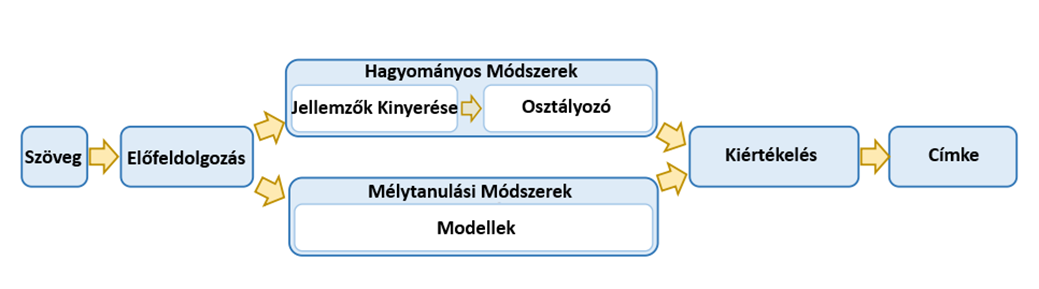
\includegraphics[width=\linewidth]{images/text_classification_flowchart}
  \caption{A szövegosztályozás tipikus folyamata: \emph{szöveg} és \emph{előfeldolgozás}, majd a \emph{hagyományos módszerek} (jellemzőkinyerés, osztályozó) és a \emph{mélytanulási módszerek} (modellek) párhuzamos ága, ezután \emph{kiértékelés} és \emph{címke} kimenet. \emph{Forrás:}~\cite{li2022surveytextclassification}.}
  \label{fig:text-classification-flow}
\end{figure}

Az osztályozási modell létrehozása előtt általában sor kerül a tanított modell \textbf{kiértékelésére} (evaluation), amely során különböző teljesítménymutatók -- például pontosság, visszahívás, F1-mérték vagy \textbf{görbe alatti terület} (Area Under the Curve, AUC) -- segítségével vizsgálható, hogy a modell milyen mértékben képes a különböző kategóriák helyes elkülönítésére. A kiértékelés elengedhetetlen lépés annak meghatározásához, hogy a modell alkalmas-e éles környezetben történő alkalmazásra, illetve hogy szükség van-e további finomhangolásra vagy alternatív jellemzők használatára.

A folyamat végén az \textbf{osztályozó} (classifier) a dokumentumot a megfelelő \textbf{címkéhez} (label) rendeli, amely a későbbi elemzési feladatok kiindulópontja lehet. A szövegosztályozás eredményei többféle további feldolgozást támogatnak, például \textbf{érzelmi állapotok feltárását} (sentiment analysis), \textbf{témaazonosítást} (topic analysis), spam- vagy anomáliaészlelést, valamint nagy szövegkorpuszok strukturálását és információvisszakeresési rendszerek hatékonyságának javítását. A címkézett adatok ezen túlmenően alapot biztosítanak prediktív modellekhez, ajánlórendszerekhez, illetve bármely olyan automatizált folyamat számára, ahol nagy mennyiségű szöveges adat gyors és megbízható kategorizálása szükséges.

\section{Áttérés a hagyományos módszerekről a mélytanulási módszerekre}

\cite{li2022surveytextclassification} szerint „az 1960-as évektől a 2010-es évekig a hagyományos szövegbesorolási módszerek domináltak” (saját fordítás), és a mélytanulási módszerekre való áttérés 2010-ben kezdődött. A hagyományos módszerek statisztikán alapulnak, és a korábbi szabályalapú módszerekhez képest nagyobb pontosságot és stabilitást mutattak. Az adatrobbanás korában azonban a manuális jellemzőkinyerés költséges és időigényes, a statisztikai megközelítések pedig figyelmen kívül hagyják a szöveges adatok természetes szekvenciális szerkezetét vagy kontextusbeli információit.

A hagyományos megközelítésekkel szemben a mélytanulási módszerek kiküszöbölik a kézzel készített szabályok és kézi jellemzőkinyerés szükségességét, mivel képesek az adatokból automatikusan, szemantikailag gazdag és kontextusérzékeny reprezentációkat tanulni. Ez a tulajdonság lehetővé teszi a \textbf{mély neurális hálózatok} (Deep Neural Network, DNN) számára, hogy olyan összetett nyelvi mintázatokat, hosszú távú függőségeket és finom szemantikai különbségeket is megragadjanak, amelyeket a hagyományos technikák jellemzően nem képesek megfelelő pontossággal modellezni. Ennek következtében a szövegosztályozás területén végzett jelenkori kutatások döntő része mély neurális hálózatokra épül, amelyek adatvezérelt architektúrákként automatikusan képesek hierarchikus jellemzők kinyerésére, és számos alkalmazási területen a legkorszerűbb teljesítményt biztosítják. Ugyanakkor a mélytanulási modellek hatékony működéséhez általában jelentős számítási kapacitásra és nagy méretű, annotált tanítóadatokra van szükség. Emiatt a \textbf{hagyományos gépi tanulási} (Traditional Machine Learning) módszerek iránti érdeklődés elsősorban azokban a szcenáriókban maradt fenn, ahol a számítási erőforrások korlátozottak, az adatmennyiség csekély, vagy valós idejű feldolgozási követelmények teszik szükségessé a könnyebb, kompaktabb modellek alkalmazását.

Két nagy osztályba sorolhatók a szövegosztályozási technikák, az \textbf{adattudomány} (Data Science) és a \textbf{mesterséges intelligencia} (Artificial Intelligence) alá~\cite{taha2024textclassificationsurvey}.

Itt érdemes megemlíteni, hogy ez a két osztály nem diszjunkt, hanem az adattudomány egy szélesebb terület, amelynek egyik eszköze lehet a mesterséges intelligencia. Ezt a következtetést definíciójukból le lehet vonni.

Az adattudomány „Olyan tudományág, amely tudományos módszereket, folyamatokat és rendszereket alkalmaz az adatokból származó ismeretek és betekintések kinyerésére”~\cite{uscensusDatascience} (saját fordítás).

A mesterséges intelligencia egyik definíciója: „Egy technológia, amely felruházza a számítógépeket és gépeket az emberi tanulás, megértés, problémamegoldás, döntéshozatal, kreativitás és önállóság utánzásának képességével”~\cite{ibmThinkAI} (saját fordítás).

\begin{figure}[htbp]
  \centering
  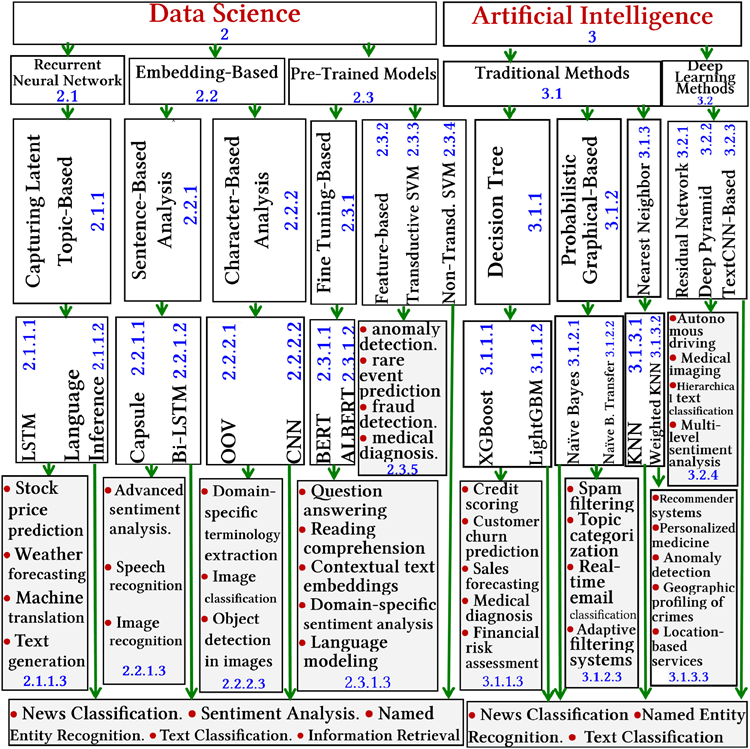
\includegraphics[width=\linewidth]{images/text_classification_taxonomy}
  \caption{A szövegosztályozási módszerek taxonómiája. \emph{Forrás:}~\cite{taha2024textclassificationsurvey}.}
  \label{fig:text-classification-taxonomy}
\end{figure}

\chapter{Előfeldolgozás}

Az előfeldolgozás fejezetben helyet kap az adathalmaz leírása, tervezés és implementálás bemutatása az adathalmaz letöltésétől egészen a tokenizált adatok mentéséig.
A tervezés a végleges változat dokumentálását fedi le, és jellegzetesebb kihívások és megoldások csak említés szintjén kerülnek megörökítésre. 
Az implementálás ötletesebb megoldások bemutatására szorítkozik, és rövid leírására az alkalmazott módszereknek.

\section{Adathalmaz eredete}

A felhasznált adathalmaz M. Wiechmann \texttt{enron\_spam\_data} GitHub-oldalán található vesszővel tagolt adatfájl 
(\texttt{CSV}) formátumban~\cite{wiechmannNoppelEnronSpam}.

Az eredeti adathalmazról, mely abban különbözik a leírtak szerint, hogy minden egyes e-mail külön fájlként van tárolva, 
a Spam filtering with Naive Bayes – Which Naive Bayes? tanulmányban olvashatunk a harmadik fejezetben. 
A következő alfejezet ezt a művet veszi alapul az adathalmaz általános bemutatására~\cite{inproceedings}.

Az Enron botrány kivizsgálásának keretében közel 150 Enron dolgozó fájljai lettek közzé téve, 
melyek között jelentős mennyiségű személyes e-mail üzenet is megtalálható. 
Személyre szabott spam filtert tűztek ki célul, így kiválasztottak 6 Enron dolgozót: 
farmer-d, kaminski-v, kirchen-l, williams-w3, beck-s és lokay-m, a Bekkerman által szolgáltatott adathalmazból, 
melyben a levelezések csak ham üzeneteket tartalmaztak ~\cite{inproceedings}.

A Spam üzeneteket négy különböző forrásból állították össze melyek sorra: a SpamAssassin corpus, a Honeypot project, 
Bruce Guenter spam gyűjteménye, és a 3. fejezet bevezetésében említett mű harmadik szerzőjének, Paliouras G. egyéni spam gyűjteménye ~\cite{inproceedings}.

A hat darab ham üzenet gyűjteményből mindegyik párba lett állítva egy spam gyűjteménnyel a három közül, 
és az arányuk három esetében 1:3-hoz lett, míg a másik három esetében 3:1-hez ~\cite{inproceedings}.

A következő előfeldolgozási műveleteket is elvégezték:
\begin{itemize}
\item Az e-mail fiók tulajdonosa által küldött levelek eltávolítása
\item HTML címkék eltávolítása
\item E-mail fejléc eltávolítása
\item Nem-latin karaktereket alkalmazó spam-ek eltávolítása
\end{itemize}

\section{Előfeldolgozás tervezése}

Egy adathalmaz előfeldolgozása során több iterációban történt az információ kinyerése az adatokról, 
majd ezen információk alapján előfeldolgozási módosítások elvégzése. A következő folyamatábra és 
leírás dokumentálja a folyamatot.
\chapter{A klasszifikációs modell és tanítási folyamat}

\section{Modelltervezés}

\subsection{BiLSTM alapú modell architektúra}

\subsection{Kimeneti réteg és veszteségfüggvény}

\subsection{Hiperparaméter-tér és optimalizálási stratégia}

\subsection{Tanítási stratégia és konvergencia elvárások}


\section{Implementáció}

\subsection{Modell implementáció (BiLSTM osztály)}

\subsection{Adatbetöltés és előfeldolgozás}

\subsection{Hiperparaméter-keresés implementációja}

\subsection{Tanítási pipeline implementáció}

\subsection{Kiértékelési metrikák implementációja}

\section{Tanítási dinamika és eredmények}

\subsection{Tanulási görbék elemzése}

\subsection{Kumulatív adathalmazon végzett tanítás hatása}

\subsection{Hiperparaméterek hatásának értékelése}
\chapter{Kísérletek és eredmények}

\section{Előfeldolgozás és tokenizálás}

\section{Hiperparaméter-optimalizálás és tanulási görbe elemzés}

\chapter{Összefoglalás és továbbhaladási irány}


% biblatex: alapból csak \cite-zett munkák jelennek meg. Az alábbi \nocite a felsorolt
% kulcsokat a Források közé teszi szövegbeli hivatkozás nélkül is (később elhagyható, ha mindenhol \cite van).
\nocite{ibmThinkNLP,wang2023textclassificationnlp,li2022surveytextclassification,taha2024textclassificationsurvey,uscensusDatascience,ibmThinkAI,kowsari2019textclassificationsurvey}
\printbibliography[heading=bibintoc,%
title=Források]
%sima bibtex verzió
%\bibliographystyle{plain}
%\bibliography{dolgozat.bib}

\pagestyle{empty}

\section*{Repository használati útmutató}

\noindent
Az alábbi útmutató a dolgozathoz tartozó repository felépítését, valamint a reprodukálhatósághoz szükséges futtatási lépéseket foglalja össze. 
A projekt GitHubon érhető el: \texttt{https://github.com/RobertFerencsik/uni-thesis}

\subsection*{Beállítás}

\begin{enumerate}
    \item CUDA-képes videokártya szükséges a futtatáshoz.
    \item Python 3.10.0 telepítése.
    \item Csomagok telepítése: \texttt{pip install -r requirements.txt}
    \item A notebookok futtatásához a Jupyter környezet és az \texttt{ipykernel} csomag telepítése is szükséges.
\end{enumerate}

\subsection*{Használat}

\subsubsection*{Adathalmaz feldolgozása}

Az adathalmaz feldolgozásához a \texttt{notebooks/} mappában található notebookokat sorrendben szükséges futtatni.

\subsubsection*{Model}

A tároló gyökerében a \texttt{main.py} a belépési pont.

\paragraph{Hiperparaméter-keresés}

\begin{verbatim}
python main.py tune [--num-trials 20]
\end{verbatim}

\noindent
A próbák száma opcionális. A reprodukálhatóság érdekében az alapértelmezett érték \textbf{20}, ezzel lett mindhárom fázis futtatva.

\paragraph{Növekményes tanítóhalmazon tanulási görbe}

\begin{verbatim}
python main.py learning-curve [--num-portions 10]
\end{verbatim}

\noindent
A részek száma szintén opcionális. Az alapértelmezés \textbf{10}. Ezzel lett kiértékelve a növekményes adathalmazokon tanított modellek \textbf{általánosító} képessége.

\subsection*{Jegyzékfa}

Az alábbi fa segít eligazodni a tárolóba. A results \textbf{jegyzék} tartalmazza a futási eredményeket, így ennek megtekintésével futtatás nélkül is tanulmányozhatóak.

\begin{small}
\begin{verbatim}
uni-thesis/
|
+-- main.py                  # Belépési pont: tune vagy learning-curve
+-- requirements.txt         # pip-függőségek
+-- README.md
+-- .gitignore               # Nem verziókezelt fájlok listája
|
+-- notebooks/
|   +-- 1-eda-1.ipynb        # EDA
|   +-- 2-data-cleaning.ipynb
|   +-- 3-verification.ipynb
|   +-- 4-tokenization.ipynb # Tokenizáló
|   +-- 5-validation.ipynb   # Validációs lépések
|   `-- (*.png)              # Futtatáskor generált ábrák
|
+-- data/
|   +-- corpora/
|   |   +-- raw/             # Enron, CSV, train/teszt/validáció
|   |   `-- processed/       # Tisztított adatok, tokenizáló tanító szöveg
|   `-- models/              
|       +-- lstm_tokenizer.model
|       +-- train_ids.pkl, train_pieces.pkl
|       +-- learning_curve/
|       |   `-- portion_01..10/
|       |       +-- best_model.pt
|       |       +-- checkpoint_epoch_*.pt
|       |       +-- eval_test_metrics.json
|       |       +-- test_confusion_matrix.png
|       |       `-- training_curves.png
|       `-- tuning/          # learning_curve-vel egyező szerkezet
|
+-- src/
|   +-- config/              # config.json, hiperparaméterek
|   +-- data/                
|   +-- models/              # bilstm.py
|   +-- training/
|   +-- evaluation/
|   +-- experiments/         # tuning.py, learning_curve.py
|   `-- infrastructure/
|
+-- thesis/                  # Szakdolgozat LaTeX
|
`-- results/
    +-- preprocessing/       # Notebookok kimenete (Markdown, ábrák)
    +-- experiements/        # Modellek kiértékelései (archívum)
    |   +-- 1_phase_one_tuning/
    |   +-- 2_phase_two_learning_curve/
    |   +-- 2_phase_two_tuning/
    |   +-- 3_phase_three_learning_curve/
    |   `-- 3_phase_three_tuning/
    `-- SPAM_HAM_uzenetek_osztalyozasa_melytanulasi_modszerekkel.pdf
\end{verbatim}
\end{small}



\end{document}
